% =============================================================================
% CHAPTER 2: LITERATURE REVIEW
% =============================================================================

\chapter{LITERATURE REVIEW}


While large language models (LLMs) are good at many tasks, their use of autoregressive generation makes them likely to produce fluent but incorrect information~\citep{ji2023survey}. For knowledge-intensive question answering, this unreliability is a major roadblock as the ability to verify reasoning against external facts is essential. To tackle this issue, recent studies have focused on grounding models in structured external facts through knowledge graphs. Still, keeping a model strictly aligned with these graphs during generation, without losing its natural flow, is a difficult challenge.

This chapter reviews the current research on these challenges and examines how knowledge graph constraints might help ensure factual accuracy during multi-hop reasoning. It outlines the connections between language model hallucination, multi-step validation, and structured grounding, and shows where soft-grounding methods do not meet expectations, highlighting the specific technical gaps this project addresses.


% -----------------------------------------------------------------------------
\section{Large Language Models and Hallucination}
\label{sec:llms}
% -----------------------------------------------------------------------------

Modern LLMs are built on the Transformer architecture~\citep{vaswani2017attention}, using scaled dot-product self-attention to weight token importance regardless of positional distance. The field has largely moved toward decoder-only models with causal masking, where each token attends only to preceding tokens. The Llama-3.1-8B model~\citep{dubey2024llama3} is a prominent example of this design and has been adopted as the backbone in recent KG-constrained decoding work~\citep{luo2025-graph-constrained-reasoning}.

Text production in these models is fundamentally autoregressive: given a vocabulary $\mathcal{V}$, an input $x$, and prior tokens $y_{<t}$, the model computes $P(y_t | y_{<t}, x)$ over the full vocabulary. Since this distribution is always defined over every token, any token has a positive, non-zero chance of being generated at any step. Decoding strategies such as beam search and nucleus sampling~\citep{holtzman2020curious} determine how a token is chosen from this distribution. This autoregressive nature creates fluent, coherent text, but since each step relies on prior outputs without an external verifier, it also directly causes hallucination.

LLMs are pretrained on vast unlabelled text using next-token prediction. The GPT series (\citealt{brown2020gpt3}; \citealt{openai2024gpt4technicalreport}) and the Llama series (\citealt{touvron2023llama}; \citealt{dubey2024llama3}) show that scaling this simple task leads to powerful downstream capabilities. During pretraining, the model internalizes patterns and facts from its training data, but this memory is fundamentally static and statistical. The model lacks a way to interact with dynamic external facts or ensure that its outputs reflect verified truths.

\subsection{Definition and Structural Causes}

Hallucination in natural language generation refers to the production of content that is fluent and internally coherent yet factually unsupported by or in contradiction with verifiable sources~\citep{ji2023survey}. \citet{huang2023survey} refine this into \textit{intrinsic hallucination} (output contradicts provided source context) and \textit{extrinsic hallucination} (output contains claims unverifiable against any source). Both types appear at non-trivial rates: \citet{ji2023survey} survey over 30 works finding hallucination rates from 15\% to over 60\%, and \citet{luo2025-graph-constrained-reasoning} report that retrieval-augmented reasoning approaches produce hallucinated reasoning steps in approximately one-third of cases even with direct access to a knowledge graph.

Hallucination is generally attributed to a combination of data, training, and inference-time factors~\citep{huang2023survey}. This work is concerned with the last of these: the autoregressive decoding mechanism itself makes hallucination structurally possible, independent of data quality or training procedure. Three properties of this mechanism are relevant. First, the generation distribution is based entirely on learned parameters, with no component that verifies tokens against an external source. Second, errors propagate forward: a hallucinated token at step $t$ becomes conditioning context for step $t{+}1$, producing fluent continuations of an incorrect chain. Third, the model imposes no hard constraint on which tokens are eligible at each step, so factually invalid continuations remain within the support of the output distribution~\citep{brown2020gpt3}.

\subsection{The Scaling Paradox}

A common argument is that larger models should eventually achieve factual reliability. Evidence does not support this. \citet{lin2022truthfulqa} introduce TruthfulQA and find that larger models do not outperform smaller ones in truthfulness and in some categories show \textit{inverse scaling}, reproducing widespread incorrect beliefs more effectively. \citet{perez2022sycophancy} show that RLHF-trained models generate confident-sounding responses aligned with apparent user expectations rather than verifiable facts. \citet{kandpal2023large} demonstrate that larger models improve on frequently-seen entity combinations but not on compositional questions requiring unseen fact combinations, precisely the structure of multi-hop KG questions. \citet{mallen2023not} confirm significant hallucination rates for GPT-4 on tail-entity questions regardless of model size. These findings establish hallucination as a structural feature of the autoregressive mechanism, not a scaling issue.

% -----------------------------------------------------------------------------
\section{Chain-of-Thought and Its Limits}
\label{sec:cot}
% -----------------------------------------------------------------------------

\subsection{Chain-of-Thought Prompting}

Chain-of-thought (CoT) prompting~\citep{wei2022cot} is the dominant paradigm for eliciting multi-step reasoning from LLMs. By including worked examples that show intermediate reasoning steps, the model learns to decompose complex problems into simpler sub-problems. \citet{wei2022cot} demonstrate accuracy improvements on arithmetic, commonsense, and multi-hop QA benchmarks, with the capability emerging at approximately 100 billion parameters. Zero-shot chain-of-thought~\citep{kojima2022zero} achieves similar benefits by adding ``Let's think step by step'' to the prompt.

Despite these improvements, CoT has a fundamental structural limitation: each intermediate step is generated by the same autoregressive mechanism. An incorrect step propagates forward as conditioning context, and no mechanism verifies that any step corresponds to a fact in an external source. A CoT chain can be entirely fluent and internally coherent while containing factually fabricated steps.

\subsection{Self-Consistency and Tree-of-Thought}

Self-consistency~\citep{wang2023selfconsistency} samples several independent CoT chains and chooses the final answer by majority vote, reducing sensitivity to individual hallucinated chains. However, a majority of independently hallucinated chains can still produce an incorrect answer, especially on deep multi-hop questions. Tree-of-Thought~\citep{yao2023-tree-of-thought} treats generation as search through a tree of partial reasoning sequences, using the LLM as both generator and evaluator. The key limitation persists: pruning decisions rely on the model's own parameters without external verification.

\subsection{Why Prompting Cannot Guarantee Faithfulness}

All prompting-based methods (few-shot, CoT, self-consistency, tree-of-thought) modify the \textit{input} to the LLM without modifying the \textit{generation mechanism}. Since decoding happens over the full vocabulary, each token has a strictly positive probability at every step. True structural faithfulness requires that invalid tokens receive exactly zero probability. This can only be achieved by directly changing the decoding algorithm~\citep{geng2023grammarconstrained, willard2023outlines}.

% -----------------------------------------------------------------------------
\section{Knowledge Graphs and Knowledge Graph Question Answering}
\label{sec:kgqa}
% -----------------------------------------------------------------------------

\subsection{Knowledge Graphs}

A knowledge graph is a structured database of verified facts, represented as directed, labelled triplets $(e, r, e')$ where $e, e' \in \mathcal{E}$ are entities and $r \in \mathcal{R}$ is a relation type. Figure~\ref{fig:kg_example} illustrates a simplified fragment of such a structure. Freebase~\citep{bollacker2008freebase}, the KG underlying the evaluation benchmarks used in this work, encodes tens of millions of triplets across geography, history, entertainment, and science~\citep{yih2016websqp, talmor2018cwq}.
\begin{figure}[H]
  \centering
  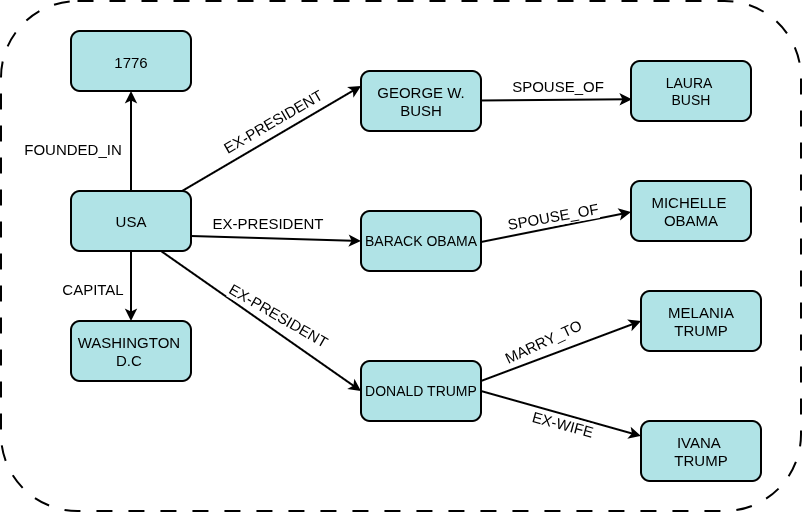
\includegraphics[width=0.8\textwidth]{Figures/kg_example.png}
  \caption[Simplified Example of a Knowledge Graph Fragment]{Knowledge Graph Fragment}
  \label{fig:kg_example}
\end{figure}

The critical distinction between a KG and an unstructured text corpus is that every triplet has been explicitly verified and is machine-readable in deterministic form. This makes KGs suitable as sources for hard constraints on generation: a candidate token can be verified via exact lookup rather than probabilistic semantic matching. A multi-hop reasoning path of length $L$ is a sequence $(e_0, r_1, e_1, \ldots, r_L, e_L)$ in which each consecutive triplet $(e_{i-1}, r_i, e_i)$ is a verified edge of $\mathcal{G}$~\citep{lan2022survey}.

\subsection{Knowledge Graph Question Answering}

KGQA requires a system to identify the answer entity $e_L$ to a natural language question $q$ by reasoning through a chain of verified KG triplets. Formally: given question $q$ with question entities $\mathcal{E}_q \subseteq \mathcal{E}$ identified by entity linking, identify the terminal entity of the correct reasoning path in $\mathcal{G}$~\citep{lan2022survey}. Early approaches relied on semantic parsing, information retrieval over KG subgraphs, or reinforcement-learning-based path traversal~\citep{das2017go}. More recent approaches use LLMs as retrievers, agents iteratively querying the KG and revising partial answers~\citep{mavromatis2022rearev}, generators conditioned on retrieved subgraph context~\citep{jiang2023structgpt, jin2024graphcot, luo2024rog}, unified retrieval-and-reasoning pipelines~\citep{jiang2022unikgqa}, or KG-infused pretrained representations~\citep{wang2021kepler}. The move toward LLM-based KGQA has improved fluency but brought back hallucination risks.

\subsection{Evaluation Benchmarks}

WebQSP~\citep{yih2016websqp} contains 4,737 questions on Freebase with reasoning depths of one to two hops, evaluated using Hits@1 and F1. ComplexWebQuestions (CWQ;~\citealt{talmor2018cwq}) builds on WebQSP through conjunction, composition, and comparative operations, resulting in about 34,000 questions requiring up to four hops. The two benchmarks stress different aspects of path selection: WebQSP questions reach the answer in one or two hops, so the valid path set stays small; CWQ questions reach up to four hops, so the valid paths are longer and correct selection depends on sustaining the right trajectory across more steps, not on filtering a larger candidate set.

\subsection{Multi-Hop Complexity}

For an entity with average out-degree $d$ in the KG, the number of valid paths of length $L$ from the question entities increases as $|\mathcal{E}_q| \times d^L$. For well-connected Freebase entities where $d \approx 20$ and a question may have up to three question entities, a three-hop question can generate up to 24{,}000 structurally valid paths, but only one leads to the correct answer~\citep{he2021improving, lan2022survey}. At each step, the model must choose the correct next token from a vast array of valid yet incorrect options.

% -----------------------------------------------------------------------------
\section{Constrained Decoding for Faithful Text Generation}
\label{sec:constrained}
% -----------------------------------------------------------------------------

Constrained decoding restricts generation to a predefined valid set at each step by directly intervening in the decoding mechanism. Unlike prompting, which changes the input to the LLM, constrained decoding alters the token selection process itself.

\subsection{Format-Constrained Decoding}

Logit masking~\citep{geng2023grammarconstrained, willard2023outlines} computes a binary mask over the vocabulary at each generation step, setting the log-probability of invalid tokens to $-\infty$ before the softmax. \citet{geng2023grammarconstrained} constrain generation to strings conforming to a context-free grammar via an Earley parser oracle. \citet{willard2023outlines} reduce the computational cost with an efficient finite-state machine (FSM) formulation, precomputing an index from automaton states to valid vocabulary subsets for amortised $O(1)$ lookup. Additional methods include Synchromesh~\citep{poesia2022synchromesh} for program synthesis, PICARD~\citep{scholak2021picard} for schema-constrained SQL parsing, NeuroLogic Decoding~\citep{lu2021neurologic} for propositional logic constraints, and GENRE~\citep{decao2021autoregressive} for trie-constrained entity retrieval. The shared limitation of all these approaches is that they enforce output \textit{format} rather than \textit{factual content}. The extension from format constraints to KG path constraints requires a constraint oracle that encodes the relational structure of the knowledge graph itself.

\subsection{Knowledge Graph-Constrained Decoding}

Applying constrained decoding to knowledge graph faithfulness uses the KG itself as the constraint oracle. At each generation step, only tokens corresponding to valid continuations of a KG reasoning path are allowed, making hallucination of KG facts structurally impossible.

\textbf{Graph-Constrained Reasoning (GCR)}~\citep{luo2025-graph-constrained-reasoning} builds a KG-Trie (a prefix tree of all KG paths within $L$ hops of the question entities, created by BFS before generation) and uses it as the constraint oracle during beam-search decoding. GCR achieves 92.6\% Hits@1 on WebQSP and 75.8\% on CWQ with 100\% structural faithfulness, using a Llama-3.1-8B backbone. The trie is created once and remains unchanged: the valid token set is fixed regardless of what has been generated.

\textbf{Decoding on Graphs (DoG)}~\citep{li2024-decoding-on-graphs} presents step-wise trie expansion as a partial solution to GCR's static oracle. After locking in an entity, the constraint trie is expanded with all KG neighbors of that entity, making the oracle topologically dynamic. DoG achieves 90.99\% Hits@1 on WebQSP and 76.08\% on CWQ with 100\% structural faithfulness. However, the expansion rule includes all KG neighbors regardless of relevance to the question, and step-wise trie construction compromises the efficiency of precomputed structures.

\textbf{RouterKGQA}~\citep{yuan2026routerkgqa} routes between a specialized KG-reasoning model and a general LLM based on question complexity. It uses SBERT embeddings (\texttt{nomic-embed-text-v1}) to filter candidate answers after generation. RouterKGQA's semantic scoring operates at the answer-selection level rather than at the token-constraint level: paths are created first and filtered afterward.

\subsection{Beam Search and Trie-Based Constraints}

Beam search~\citep{lowerre1976harpy, holtzman2020curious} keeps the $k$ most promising partial hypotheses at each step, reducing early-error multiplication. A prefix trie~\citep{fredkin1960trie, willard2023outlines} yields the valid next-token subset in $O(1)$ time. GCR's KG-Trie~\citep{luo2025-graph-constrained-reasoning} serializes verified multi-hop paths from the KG into string format mapped to the LLM's token vocabulary. When beam search is merged with a KG-Trie oracle, the decoding process becomes a strictly bounded traversal of the prefix tree: at each autoregressive step, the current beam hypotheses map to specific trie states, and a mathematical mask forces the probability of any token not present as a child node to zero. The beam search then advances strictly down permissible branches.

% -----------------------------------------------------------------------------
\section{Retrieval and Soft Grounding}
\label{sec:rag}
% -----------------------------------------------------------------------------

Retrieval-augmented generation (RAG)~\citep{lewis2020rag} is the leading approach for grounding LLM outputs in external knowledge. A dense retriever selects relevant passages based on embedding similarity, and a reader LLM generates the answer from the retrieved context. Fusion-in-Decoder~\citep{izacard2021leveraging} enhances this by encoding multiple passages separately and merging them in the decoder. Self-RAG~\citep{asai2024selfrag} adds reflection tokens for when to retrieve and whether passages support claims. FLARE~\citep{jiang2023flare} triggers retrieval when next-token confidence drops. IRCoT~\citep{trivedi2022ircot} interleaves retrieval with CoT steps, improving multi-hop accuracy. GraphRAG~\citep{edge2024graphrag} builds community-structured KGs from document collections for complex relational queries.

In the KGQA context, several approaches enhance RAG with structured context. \citet{he2021improving} retrieve KG subgraphs with attention-guided traversal. \citet{yasunaga2021qagnn} combine text passages and KG neighborhoods through graph neural networks. \citet{shi2021kgpath} retrieve KG paths as natural language context strings. Sentence-BERT~\citep{reimers2019sbert} encoders produce dense vector representations where cosine similarity proxies semantic alignment, applied in these systems to rank candidate KG paths as soft retrieval signals~\citep{shi2021kgpath, saxena2022kgqa}.

\subsection{The Structural Limitation of Soft Grounding}

Despite their empirical improvements, all RAG approaches share a structural limitation: retrieved context is a soft influence on generation. The retriever determines what the LLM sees; it does not determine what the LLM is permitted to generate. Because the generation mechanism remains unchanged, there exists a nonzero probability of generating any token at any step, including tokens that correspond to no verified KG fact. Structural faithfulness with probability one cannot be achieved under any architecture that modifies only the input context without modifying the token selection mechanism~\citep{luo2025-graph-constrained-reasoning, geng2023grammarconstrained}.

% -----------------------------------------------------------------------------
\section{Unresolved Gaps}
\label{sec:synthesis}
% -----------------------------------------------------------------------------

The review shows that two different research paths, constrained decoding for structural faithfulness and semantic similarity for relevance-guided reasoning, have developed mainly in parallel without being combined at the constraint-oracle level. Constrained decoding methods~\citep{luo2025-graph-constrained-reasoning, li2024-decoding-on-graphs} achieve structural faithfulness but create their constraint oracles without considering question semantics or the context of generation. This leads to valid token sets that include many irrelevant paths. Semantic similarity methods~\citep{shi2021kgpath, saxena2022kgqa, yuan2026routerkgqa} improve relevance but act as soft signals that affect retrieval or selection after the fact, without changing the generation process.

Three specific gaps emerge from this review.

\textbf{Gap 1: The Permissiveness Problem.} Current KG-constrained decoding frameworks build their constraint oracles based on graph structure and question entities only. They do not consider question semantics or the current generation state. In the case of multi-hop questions, this results in valid token sets with thousands of structurally correct but semantically irrelevant paths at each generation step. The LLM has to sort through these paths using its own knowledge, which reintroduces the risk of hallucination that constrained decoding aimed to eliminate~\citep{luo2025-graph-constrained-reasoning, li2024-decoding-on-graphs}.

\textbf{Gap 2: The Static-Dynamic Efficiency Tradeoff.} GCR's precomputed static trie is efficient in computing but lacks semantic awareness and remains the same at every generation step. DoG's step-wise topological expansion adds some dynamism but requires reconstructing the trie at every step and does not include semantic filtering~\citep{li2024-decoding-on-graphs, willard2023outlines}. No current framework achieves semantic responsiveness, where the valid set narrows progressively as reasoning moves in a specific direction, while also maintaining the efficiency of precomputed constraint structures.

\textbf{Gap 3: The Absence of a Constraint Quality Metric.} No existing work offers a metric that measures constraint permissiveness separately from the accuracy of downstream answers. Without this metric, it is not possible to track progress on reducing irrelevant paths in the valid set or to compare frameworks based on constraint quality without factoring in model quality.

Table~\ref{tab:related_summary} summarizes the key works reviewed in this chapter, categorizing them by their approach, whether they provide structural faithfulness guarantees, and whether they incorporate semantic conditioning into their constraint mechanisms.

\begin{longtable}[htpb]{|>{\raggedright\arraybackslash}p{3.5cm}|>{\raggedright\arraybackslash}p{4cm}|>{\raggedright\arraybackslash}p{3cm}|>{\raggedright\arraybackslash}p{3cm}|}
  \caption[Summary of Key Related Works]{Summary of Key Related Works} \label{tab:related_summary}                                                   \\
  \hline
  \textbf{Work}                               & \textbf{Approach}                & \textbf{Structural Faithfulness} & \textbf{Semantic Conditioning} \\
  \hline
  \endfirsthead

  \hline
  \textbf{Work}                               & \textbf{Approach}                & \textbf{Structural Faithfulness} & \textbf{Semantic Conditioning} \\
  \hline
  \endhead

  \hline
  \endfoot

  \hline
  \endlastfoot

  \citet{luo2025-graph-constrained-reasoning} & Static KG-Trie decoding          & Yes (100\%)                      & No                             \\ \hline
  \citet{li2024-decoding-on-graphs}           & Step-wise topological expansion  & Yes (100\%)                      & No                             \\ \hline
  \citet{yuan2026routerkgqa}                  & Routing + post-hoc filtering     & Probabilistic                    & Yes (answer-level)             \\ \hline
  \citet{luo2024rog}                          & Reasoning path planning          & No                               & Partial                        \\ \hline
  \citet{jiang2023structgpt}                  & LLM over structured data         & No                               & Partial                        \\ \hline
  \citet{jin2024graphcot}                     & Graph-augmented CoT              & No                               & Partial                        \\ \hline
  \citet{jiang2022unikgqa}                    & Unified retrieval and reasoning  & No                               & Partial                        \\ \hline
  \citet{wang2021kepler}                      & KG-pretrained language model     & No                               & Partial                        \\ \hline
  \citet{mavromatis2022rearev}                & Iterative reasoning revision     & No                               & Partial                        \\ \hline
  \citet{he2021improving}                     & KG subgraph attention            & No                               & Partial                        \\ \hline
  \citet{yasunaga2021qagnn}                   & Text-KG graph neural network     & No                               & Partial                        \\ \hline
  \citet{das2017go}                           & RL-based KG path traversal       & No                               & Soft                           \\ \hline
  \citet{saxena2022kgqa}                      & Embedding-based path selection   & No                               & Soft                           \\ \hline
  \citet{shi2021kgpath}                       & Path retrieval by similarity     & No                               & Soft (retrieval)               \\ \hline
  \citet{asai2024selfrag}                     & Retrieval with reflection        & No                               & Soft                           \\ \hline
  \citet{edge2024graphrag}                    & Community-structured retrieval   & No                               & Soft                           \\ \hline
  \citet{geng2023grammarconstrained}          & Grammar-constrained decoding     & Format only                      & No                             \\ \hline
  \citet{willard2023outlines}                 & FSM-indexed constrained decoding & Format only                      & No                             \\ \hline
  \citet{decao2021autoregressive}             & Entity trie-constrained decoding & Entity names only                & No                             \\ \hline
  \citet{scholak2021picard}                   & Schema-constrained SQL parsing   & Schema only                      & No                             \\ \hline
  \citet{lu2021neurologic}                    & Logic-constrained decoding       & Format only                      & No                             \\
\end{longtable}

These three gaps collectively identify an open problem at the intersection of the two research trajectories reviewed in this chapter: integrating semantic relevance scoring directly into the constraint oracle, conditioning the valid token set jointly on the knowledge graph, the question semantics, and the evolving generation state.
